\documentclass[11pt,a4paper]{article}
\usepackage[fleqn]{amsmath}
\usepackage{amssymb,latexsym}
\usepackage[colorlinks=true,linkcolor=black,citecolor=black,urlcolor=black]{hyperref}
\usepackage{tikz,color}

\begin{document}

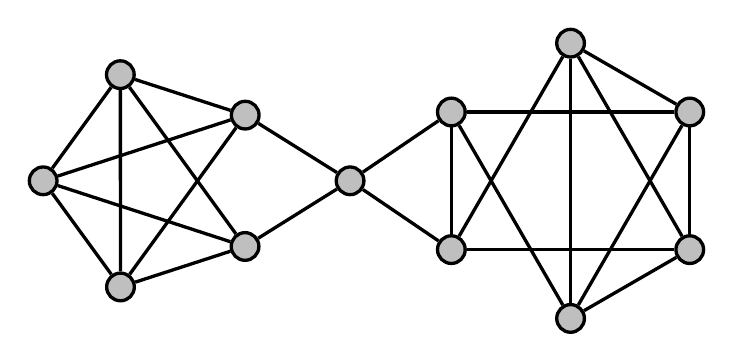
\begin{tikzpicture}[x=0.2mm,y=0.2mm,very thick,vertex/.style={circle,draw,minimum size=10,inner sep=0,fill=lightgray}]
	\node at (-164.2,67.4) [vertex] (v1) {};
	\node at (197.4,43.7) [vertex] (v2) {};
	\node at (46,-43.7) [vertex] (v3) {};
	\node at (-213.2,0) [vertex] (v4) {};
	\node at (121.7,-87.4) [vertex] (v5) {};
	\node at (-18.3,0) [vertex] (v6) {};
	\node at (-164.1,-67.4) [vertex] (v7) {};
	\node at (121.7,87.4) [vertex] (v8) {};
	\node at (-84.9,41.7) [vertex] (v9) {};
	\node at (-85,-41.7) [vertex] (v10) {};
	\node at (46,43.7) [vertex] (v11) {};
	\node at (197.4,-43.7) [vertex] (v12) {};
	\draw (v1) to (v4);
	\draw (v1) to (v7);
	\draw (v1) to (v9);
	\draw (v1) to (v10);
	\draw (v2) to (v5);
	\draw (v2) to (v8);
	\draw (v2) to (v11);
	\draw (v2) to (v12);
	\draw (v3) to (v6);
	\draw (v3) to (v8);
	\draw (v3) to (v11);
	\draw (v3) to (v12);
	\draw (v4) to (v7);
	\draw (v4) to (v9);
	\draw (v4) to (v10);
	\draw (v5) to (v8);
	\draw (v5) to (v11);
	\draw (v5) to (v12);
	\draw (v6) to (v9);
	\draw (v6) to (v10);
	\draw (v6) to (v11);
	\draw (v7) to (v9);
	\draw (v7) to (v10);
	\draw (v8) to (v12);
\end{tikzpicture}

\end{document}